\documentclass[12]{article}
\usepackage[spanish,english]{babel}
%\usepackage[spanish]{babel}
\usepackage[utf8]{inputenc}
\usepackage{graphicx}
\usepackage{epsfig}
\usepackage{multirow}
\usepackage{multicol,caption}
\usepackage{amsthm} % Theorem Formatting
\usepackage{amssymb}    % Math symbols such as \mathbb
\usepackage{color}
\usepackage{hyperref}
\usepackage[none]{hyphenat}
\usepackage{appendix}
\renewcommand{\appendixname}{Anexo}
\renewcommand{\appendixtocname}{LISTA DE ANEXOS}
\renewcommand{\appendixpagename}{Anexos}
%\renewcommand{\tablename}{Tabla}
%\def\tablename{Cuadro}% por \def\tablename{Tabla}% 
\newenvironment{Figure}
{\par\medskip\noindent\minipage{\linewidth}}
{\endminipage\par\medskip}
\addto\captionsspanish{%
\def\tablename{Tabla}%
}
\topmargin  = 10pt
\oddsidemargin  = -0.5in
%\headheight = 12pt
%\headsep    = 15pt
%\footskip   = 15pt
\textheight = 21.5 cm
\textwidth  = 18.5cm
\tolerance=10000
\title{\bf{Ilustración de la ley del cuadrado inverso de la densidad de flujo de radiación emitida por un diodo led emisor infrarrojo, utilizando el modulo motorizado infrarossi y su software de control Free infrarossi}}
\author{Julian Salamanca\footnote{jasalamanca@udistrital.edu.co}, Diego Parra\footnote{diegoestudianteud1@gmail.com} \\
  Universidad Distrital, Calle 3 No 26A-40 Bogotá-Colombia\\
  Grupo de Física e Informática ``FISINFOR''
}
\date{\today}
\begin{document}
%\def\tablename{Cuadro}% por \def \tablename{Tabla}% 
\renewcommand{\tablename}{Tabla}
\maketitle
\vspace{-0.8cm}
\selectlanguage{english}
\begin{abstract}
The present article illustrates the attenuation due to the inverse square law of the flux of radiation emitted by a LED diode infrared emitter, using a mirror, the motor module  infrarossi and control software free infrarossi, environment GNU- linux; highlighting the functionality of this instrument  illustration attenuation because to the irradiansa in point source is proportional to the inverse of the distance squared if not consider other types of attenuation, this is a property of the electromagnetic waves and its duality wave - quantum.\\
{\bf{Keywords:}} Motor module, infrared sensors, microcontroller module bluetooth, electromagnetic wave, attenuation, inverse square law.
\selectlanguage{spanish}
\begin{center}
{\bf{Resumen}} 
\end{center}
El presente trabajo ilustra la atenuación debido a la ley del cuadrado inverso de la densidad de flujo de radiación emitida por un diodo led emisor infrarrojo, utilizando un espejo, el modulo motorizado  infrarossi y su software de control free infrarossi, en un entorno GNU-linux; resaltando la funcionalidad de este instrumento en la ilustración de la atenuación debido a que la irradiansa de una fuente puntual es proporcional al inverso de su distancia al cuadrado si no se consideran otros tipos de atenuación, esta es una  propiedad de la ondas electromagnéticas y su dualidad onda – quantum. \\
{\bf{Descriptores:}} Modulo motorizado, sensores infrarrojos, microcontrolador, modulo bluetooth, ondas electromagnéticas, atenuación, ley del cuadrado inverso, quantum. 
\end{abstract}
%tabla de contenido sin numeracion
%\renewcommand\contentsname{\centering TABLA DE CONTENIDO}
%\thispagestyle{empty}
%\setcounter{page}{1}
%\tableofcontents
%\clearpage
%lista de figuras
%\renewcommand\listfigurename{\centering LISTA DE FIGURAS}
%\listoffigures
%\clearpage
%lista de tablas
% \renewcommand\listtablename{\centering LISTA DE TABLAS}
% \listoftables
% \clearpage
\begin{multicols}{2}
\section{Introducción}
Los fenómenos de las ondas siempre han fascinado nuestros pensamientos y tratamos de acercarnos a estos fenómenos para tratar de entenderlos, es allí donde la física con ayuda de la matemática muestran su majestuosidad, al explicar de manera muy detallada estos fenómenos de transporte; la atenuación es una de estas propiedades, la cual esta muy presente en la vida diaria y con la ayuda del modulo motorizado infrarossi y su software de control free infrarossi, se ilustra este fenómeno físico y se realiza un calculo del valor exponencial de la distancia a la cual se atenua la irradiansa propia producida por un diodo infrarrojo emisor. \\ \\
``Una fuente de luz casi siempre ilumina la superficie de los objetos desigualmente. Así, una lámpara suspendida sobre una mesa ilumina mejor el centro de ésta. Los bordes de la mesa están mucho menos iluminados. Esto no sólo se debe a que la intensidad de la luz de la lámpara eléctrica sea distinta en diferentes direcciones. Incluso en el caso un foco puntual corresponderá a la superficie del centro más potencia luminosa (flujo luminoso)  que a una superficie igual en el borde. \\
Se llama iluminación (o iluminancia ) a la razón del flujo luminoso, que incide sobre una superficie determinada, al área de dicha superficie. \\ 
Como unidad de iluminación se toma el lux (lx); un lx es la iluminación con la cual sobre 1 metro cuadrado de superficie se distribuye uniformemente un flujo luminoso de un lumen. \\ \\
La dependencia de la iluminacion respecto de la distancia a la fuente se puede determinar colocando mentalmente una fuente puntual en el centro de una esfera, la iluminación sera igual al flujo luminoso total de la fuente distribuido sobre el área de la esfera. \\ \\
Es decir, la iluminación de una superficie es inversamente proporcional al cuadrado de su distancia a la fuente. "\cite{FISICA4}
\selectlanguage{spanish}
\section{Marco teórico}
Los fotones producidos por el diodo emisor de la fuente emisora de radiación infrarroja se dan debido a que “en los semiconductores, con estructura compleja de las bandas energéticas, son posibles las transiciones indirectas de los electrones de la banda de conducción  a la de valencia acompañadas de la emisión de un fotón. En este caso la recombinación del electrón libre con el hueco se desarrolla con la aparición de un fonón, lo que asegura la conservación del cuasi impulso. Lo más probable es que el fonón sea emitido. Si en el semiconductor se desarrollan procesos de recombinación entre bandas  tanto directa como indirectas, en el espectro de radiación se observan dos bandas de luminiscencia. \\ \\
En la banda prohibida de los semiconductores reales existe una gran cantidad de estados localizados, que están ligados a los átomos de impureza, defectos de la estructura, infracciones de la periodicidad de la estructura en la superficie, etc. Estos estados localizados desempeñan un papel importante  en los procesos de luminiscencia. \\ \\
Las transiciones de los electrones de la banda de conducción a los niveles de los pequeños donadores (o de los huecos de la banda de valencia a los niveles de los pequeños aceptores),  que hacen que estos últimos se neutralicen, pueden ser con radiación.. En este caso es de esperar la aparición de luminosidad en la región infrarroja remota del espectro. Pero los cálculos  muestran que en estas transiciones lo más probable es que sea emitido un fonón y no un fotón, es decir, que el proceso se desarrolla sin radiación. La recombinación con radiación se produce por lo general  como viene mostrado en la figura 1. Primero un electrón de la banda de conducción es capturado por un nivel local situado un poco más abajo que Ec  \footnote{Ec es el nivel de energía de conducción.}, y después se efectúa la recombinación de este electrón localizado con un hueco de la banda de valencia, la cual va acompañada de la emisión de un fotón. El electrón puede también realizar una transición con radiación de la banda de conducción y después recombinarse con un hueco. \\
\begin{Figure}	
\center
\begin{tabular}{|l|r|}
\hline
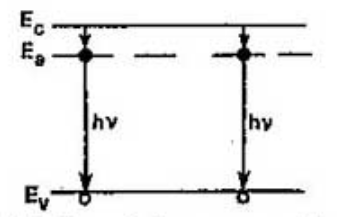
\includegraphics[width=6cm, height=6cm]{img/transiciones.png} \\ \hline
\end{tabular}
\captionof{figure}{Transiciones con radiación entre una banda y los estados de impureza.}
\label{fig:g1}
\end{Figure}
El estudio de los espectros de luminiscencia relacionados a diversas impurezas y defectos permite obtener información sobre estas infracciones de la estructura. \\ \\
Durante la absorción de la luz puede surgir en los semiconductores pares electrón – hueco ligados por la atracción coulombiana, es decir, excitones. Si uno de estos pares se aniquila, se produce la emisión de un fotón. La energía de esta radiación es: 
\begin{equation}
h\nu = E_g - E,
\end{equation}
donde E es la energía de enlace del excitón." \cite{SEMICONDUCTOR} \\ \\
Ahora se tiene un flujo de fotones de energía $h\nu$ saliendo del diodo emisor infrarrojo,  ``como los fotones viajan a la velocidad de la luz deben, de acuerdo con la teoría de la relatividad, tener una masa en reposo igual a cero; de aquí que su energía sea completamente cinética. Si un fotón existe, entonces se mueve a la velocidad de la luz, $c$; si deja de moverse a velocidad c, deja de existir. Para $m_{0} = 0$ la relación relativista momentum – energía  se convierte en $E = pc$.
de esta forma, cada fotón tiene un momentum de 
\begin{equation}
p = \frac{E}{c} = \frac{h\nu}{c} = \frac{h}{\lambda}
\end{equation}
Desde el punto de vista cuántico, un haz de energía electromagnética se compone de fotones que se desplazan a la velocidad $c$. La intensidad del haz será proporcional al número de fotones que cruza un área unitaria por unidad de tiempo. Entonces, si el haz es monocromático (de una frecuencia), la intensidad $I$ se obtendrá de 
\begin{equation}
I = (h\nu)\times \left ( \frac{N}{S\times t } \right)
\end{equation}
$h$ es la constante de Plank que tiene un valor de $6.626 \times 10^{-34} (J * s)$; $N$ es el número de fotones que pasan por segundo a través de la superficie; $S$ es la superficie; $t$ es el tiempo en segundos."\cite{FISICA_MODERNA}\\ \\
Esta radiansa de fotones desde el diodo emisor, avanza por el espacio proyectando un ángulo solido, por lo que la irradiansa  sera igual al cociente de la radiansa con el ángulo solido proyectado.\\\\
La maxima distancia que se toma para la radiansa de fotones es de 24 centimetros desde el diodo emisor hasta un espejo colocado perpendicular al flujo de energía; el vehículo motorizado infrarrojo avanza 2 milímetros por cada paso, recolecta 140 datos por cada avance y avanza 117 veces.\\ \\
El flujo de fotones que interactua con la superficie cuasi especular del espejo dan como resultado un fenómeno físico llamado reflexión, mirando el fenómeno desde el punto de vista clásico, el flujo de fotones  es  visto como el flujo de ondas electromagnéticas,   las que interactúan con la materia  en donde parte de la energía es transmitida al material aumentando la energía cinética media de sus constituyentes, y el resto del flujo electromagnético avanza paralelamente contrario a la dirección de desplazamiento inicial, si no se considera interacción de las ondas electromagnéticas con el aire como medio disipativo  y otras formas de perdida de energía; el frente de onda tiene que avanzar nuevamente 24 centímetros hasta el detector, lo que habrá avanzado desde el emisor hasta el detector el doble de la distancia que del emisor al espejo, este paso se realiza varias veces reduciendo la distancia de separación de la fuente al receptor (cuando el vehículo infrarossi avanza).\\\\
Como la irradiansa es proporcional al inverso del cuadrado de la distancia (suponiendo una fuente puntual y homogénea), la intensidad de información energética decrecerá también con el cuadrado de la distancia, haciendo que en el sensor sea menor la presión de radiación o en otras palabras la cantidad de fotones se reducirá con el inverso del cuadrado de la distancia.\\\\
Al iluminar el diodo receptor infrarrojo con esta energía radiante, ``en el semiconductor por cada fotón absorbido se rompe un enlace y se crea un par electrón-hueco. 
Es importante destacar que no todos los portadores fotogenerados contribuyen a la conducción, ya que una fracción importante de ellos se recombinan antes de llegar al extremo correspondiente del semiconductor. El calculo del incremento de corriente $\Delta I_{e}$, debida al exceso de electrones generados en la banda de conducción, $\Delta n$, es
\begin {equation}
\Delta I_{e} = q\mu _{e}(\Delta n)ES
\end{equation} 
siendo $E$ el campo eléctrico aplicado, $\mu_{e}$ la movilidad de los electrones y $S$ la sección transversal del fotoconductor.\\\\
En condiciones de iluminación, el estado estacionario se alcanza cuando la velocidad de generación de portadores en todo el volumen del semiconductor, $G$, se iguala a la velocidad de recombinación, $R$, es decir $R = G$. para un conductor intrínseco en el cual existe un exceso de portadores, $\Delta n = \Delta p$, la velocidad de recombinación de los portadores vendrá dada por:
\begin{equation}
R = \frac{\Delta n }{\tau} = \frac{\Delta p}{\tau}
\end{equation}
siendo $\tau$ el tiempo de vida media de los portadores fotogenerados. En un semiconductor de longitud $L$ en el que suponemos que el espesor es suficiente para que toda la luz que incide sobre el, sea absorbida en su interior, se tiene ahora para la velocidad de generación de portadores en la banda de conducción:
\begin{equation}
G = \eta n_{fot} = \eta \frac{\frac{P_{i}}{h\nu}}{SL}
\end{equation}
siendo $n_{fot}$ el número de fotones incidentes en el semiconductor por unidad de volumen y de tiempo, y $\eta$ la eficiencia de la conversión en la generación de portadores. El valor $n_{fot}$ se calcula a través del cociente entre la potencia de la luz incidente, $P_{i}$, y la energía de la radiación, $h\nu$, dividido a su vez por el volumen del material.\\ \\
Sabiendo que la velocidad de arrastre de los electrones por el campo eléctrico viene dada por: $v_{e} = \mu_{e}E$, las igualdades anteriores permiten escribir para la corriente de electrones fotogenerada entre los dos electrodos:
\begin{equation}
\Delta I_{e} = q\nu_{e}\eta\frac{\frac{P_{i}}{h\nu}}{L}\tau
\end{equation}
si se tiene en cuenta que el cociente $t_{r} = L/v_{e}$, representa el tiempo de trásito de los electrones entre los dos electrodos, resulta para $\Delta I_{e}$:
\begin{equation}
\Delta I_{e} = q\eta \frac{P_{i}}{h\nu}\frac{\tau}{t_{r}}
\end{equation}
con una expresión similar para la corriente de huecos en la banda de valencia. En la ecuación anterior, el factor $q\eta(P_{i}/h\nu) = I_{fot}$ tiene dimensiones de corriente y representa la velocidad de generación de carga en el semiconductor. En función de este parámetro, se define el factor de ganancia del fotoconductor a través del cociente:
\begin{equation}
\frac{\Delta I}{I_{fot}} = \frac{\tau}{t_{r}}
\end{equation}
ahora bien un diodo operando con cierto voltaje aplicado, $V$, en presencia de radiación electromagnética  capaz de excitar portadores a través de la banda prohibida dejara pasar una intensidad I dada por:
\begin{equation}
I = I_{0}[e^{(qV/kT)}-1] - I_{L}
\end{equation}
donde $I_{0}$ representa la corriente típica de un diodo, $I_{L}$ representa la corriente debida a  los portadores generados. El valor de $I_{L}$ puede calcularse de la siguiente manera:
\begin{equation}
I_{L} = qGS(L_{e} - L_{h})
\end{equation}
siendo $G$ el número de portadores generados por unidad de volumen y de tiempo y $S$ el área de la sección transversal del diodo. $L_{e}$ y $L_{h}$ representan las longitudes de difusión de los electrones y huecos. El dispositivo funciona entonces como detector del nivel de iluminación  convirtiendo una señal óptica en señal eléctrica." \cite{FOTOELECTRICO}\\ \\ 
Como la corriente I en el diodo es proporcional a la irradiansa de la superficie iluminada por fotones infrarrojos y esta ultima se atenúa con el inverso del cuadrado de la distancia del frente de energía a la fuente; en otras palabras como el voltaje que mide el microcontrolador es directamente proporcional a la corriente $I$ en el diodo receptor infrarrojo, por consiguiente el voltaje medido en el semiconductor debe  tener una relación inversamente proporcional al cuadrado de la distancia.
\begin{equation}
V(x) = \frac{A_{0}}{x^{2}}
\end{equation}
%----------------------aca empieza el montaje experimental-------------------------
\section{Montaje experimental}
\subsection{Materiales del montaje}
Para la realización de este montaje se utilizarón los siguientes materiales:
\begin{enumerate}
\item[a.] Ordenador con sistema operativo GNU-Linux.
\item[b.] Modulo motorizado infrarossi.
\item[c.] Software de control free infrarossi.
\item[d.] Espejo de 10x20 $cm^{2}$.
\item[e.] Modulo bluetooth para pc.
\end{enumerate}
\subsection{Montaje}
Situar el vehículo motorizado infrarossi a una distancia de 24 cm del espejo tal como se muestra en la figura 2, el espejo debe estar perpendicular a la parte frontal del vehículo. Abrir una terminal de GNU-Linux y escribir infrarossi, oprimir enter y la clave de superusuario, luego de abrir el programa debe oprimir el boton on, esperar que se empareje el bluetooth, una vez emparejado el bluetooth el programa desplegara un tercer menú, oprimir el botón de atenuación y esperar que el programa tome los datos necesarios. 
\begin{Figure}	
\center
\begin{tabular}{|l|r|}
\hline \\
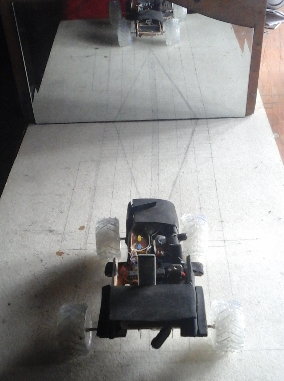
\includegraphics[width=5cm, height=6cm]{img/mon_ate.png} \\\\ \hline
\end{tabular}
\captionof{figure}{Imagen del montaje para la atenuación utilizando el modulo motorizado infrarossi y un espejo.}
\label{fig:g2}
\end{Figure}
Luego de capturar los datos, aparecerá la gráfica de esstos, los cuales se aprecian en la figuara 3, esta ya contiene el análisis estadístico y arroja el valor del exponente que debe tener la distancia. La gráfica de análisis y los datos capturados se almacenan dentro del archivo llamado Carpetas/Atenuacion con la fecha y hora del análisis de datos.
\begin{Figure}	
\center
\begin{tabular}{|l|r|}
\hline
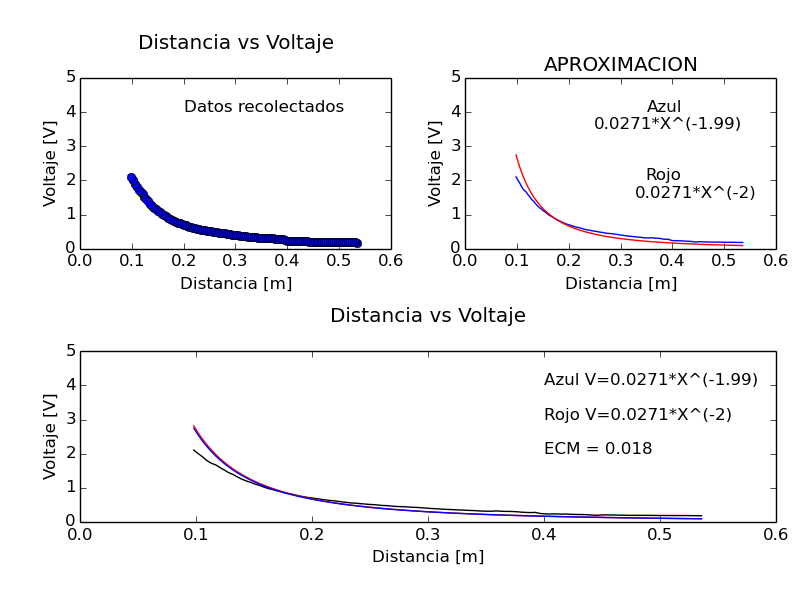
\includegraphics[width=8cm, height=6cm]{img/Atenuacion.png} \\ \hline
\end{tabular}
\captionof{figure}{Imagen generada por el programa free infrarossi, donde se aprecia la gráfica de los datos capturados en el experimento de atenuación en puntos azules, las gráficas con la linea de color azul es la gráfica estimada estadísticamente, las gráficas con las lineas de color rojo es la gráfica teórica.}
\label{fig:g3}
\end{Figure}
\section{Análisis de resultados}
El programa free infrarossi después de terminar de recoger los datos realiza un análisis estadístico de los mismos con un “ajuste lineal de una función exponencial de la forma $Y^{*} = aX^{b}$, siendo $Y$ la variable dependiente, $a$ la amplitud, $X$ la variable independiente,  $b$ el valor del exponente en este caso de atenuación, $Y^{*}$ es el valor esperado de la variable dependiente; aplicando logaritmo natural para linealizar se obtiene:
\begin{equation}
ln ( Y^{*}) = ln (a) + bln(X)  \cdots \Longrightarrow V^{*} = A + bU
\end{equation} 
donde $V^{*}$ es $ln(Y^{*})$, $A $ es el $ln(a)$ y $U$ es igual al $ln(X)$. \\\\
La suma de  todos los errores debe ser diferentes a cero $\sum e \neq 0$. \\
El exponente de ajuste b se halla con la varianza de $U$ sobre $V$  dividida entre la varianza de $U$ sobre $U$, obteniendo
\begin{equation}
b = \frac{S_{UV}}{S^{2} _{U}} =  \frac{\frac{1}{n} \sum_{i=1}^{n} UV - \bar{U} \bar{V}}{\frac{1}{n} \sum _{i=1}^{n} U^{2} - \bar{U}^2}
\end{equation}
ahora el valor de A sera igual al valor medio del logaritmo de la variable dependiente $\bar{V}$ menos el valor de la multiplicación entre el exponente $b$ y el valor medio del logaritmo de la variable independiente:
\begin{equation}
A = \bar{V} -b\bar{U}
\end{equation}
deshaciendo el logaritmo de $A$  se obtiene el valor de la amplitud a:
\begin{equation}
a = antiln(A) = antiln(\bar{V} – b\bar{U})
\end{equation}
de modo que el ajuste efectuado es:
\begin{equation}
Y^{*} =  aX^{b}  = [antiln(\bar{V} - b\bar{U})]*X^{ \left(\frac{\frac{1}{n} \sum_{i=1}^{n} UV - \bar{U} \bar{V}}{\frac{1}{n} \sum _{i=1}^{n} U^{2} - \bar{U}^{2}}\right)}
\end{equation}
la bondad del ajuste es el error cuadrático medio o $ECM$ y es igual a: 
\begin{equation}
ECM = \frac{\sum_{i=1}^{n}e_{i}^{2}}{n}
\end{equation}
siendo $e_{i}$ cada una de las diferencias entre las variables dependientes y los valores estimados para las variables dependientes $e_{i} = Y_{i} - Y^{*}_{i}$; al haber transformado la variable dependiente ya no se minimiza $\sum e^{2}$ sino $\sum (ln(Y) – ln(Y^{*}))^{2}$, de ahí que $\sum e \neq 0$."\cite{ESTADISTICA}\\\\
En la tabla 1, se muestra los resultados obtenidos después de seis pruebas del exponente de atenuación con el modulo motorizado infrarossi y su software de control free infrarossi; en ella se observa que la amplitud de la función tiene un valor medio de 0,0277, el valor medio del factor de atenuación de la distancia es -1,992; el valor obtenido en el análisis estadístico esta muy próximo al valor teórico; por lo que queda demostrado que la cantidad de energía radiada por el diodo emisor decrece con el inverso del cuadrado de la distancia. \\ \\
\begin{center}
\begin{tabular}{|c|c|c|c|c|} 
\hline
\bf{Prueba} & \bf{a} & \bf{b} & \bf{teorico} & \bf{ECM} \\
\hline
 1 & 0.027 & -2,067 & -2 & 0.124\\
\hline
 2 & 0.0276 & -2.081 & -2 & 0.054\\
\hline
 3 & 0.0291 & -1.863 & -2 & 0.077\\
\hline 
 4 & 0.0276 & -2.008 & -2 & 0.044\\
\hline
5 & 0.0282 & -1.939 & -2 & 0.051\\
\hline
6 & 0.0271 & -1.99 & -2 & 0.018\\
\hline
\end{tabular}
\\
\end{center}
\textbf{Tabla 1.} Datos obtenidos de seis pruebas para medir el exponente de atenuación, con el modulo motorizado infrarossi y su software de control free infrarossi; $a$ es la amplitud de la función, $b$ es el exponente con el que se atenúa la función, $ECM$ es el error cuadrático medio, o también llamado bondad en el ajuste. \\ \\ 
Por tanto el Voltaje en función de la distancia tiene una ecuación estimada de:
\begin{equation}
V(x) = 0,0277 X^{-1,99} 
\end{equation}
\section{Conclusiones}
\begin{enumerate}
\item[*] El modulo motorizado infrarossi y su software de control ilustran de manera cuantitativa y cualitativa fenómenos ondulatorios y corpusculares  de la radiación electromagnética como la atenuación con el inverso del cuadrado de la distancia, la radiansa, la irradiansa, fenómenos de transporte e  inyección y su análisis estadístico, calculando de una manera aproximada el exponente que acompaña a la atenuación debido a la distancia de propagación del flujo de energía radiante producida en el diodo emisor infrarrojo.   
\item[*] El modulo motorizado infrarossi y su software de control es una herramienta fácil de usar y muy precisa, capaz de ser utilizada para diversos propósitos en el aula de clase como modelo pedagógico,  tanto de profesionales como estudiantes de ciencias exactas.
\item[*] La física que se encuentra de manera implícita y explicita en este trabajo hace que el instrumento motorizado infrarossi y su software de control free infrarossi sea un herramienta indispensable  en el aula de clase en el momento de enseñar las  propiedades de las ondas electromagnéticas y los fenómenos físicos – cuánticos  que acompaña el mundo de los materiales  semiconductores.
\end{enumerate}
% ---------------------Aca empieza la bibliografia----------------------------------------------
\begin{thebibliography}{99}
\bibitem{FISICA4} Miákishev, G. (1995). Bujovsev. Física 4. Editorial Mir Moscú. Moscú. 198658. Frumento A. Biofísica.
\bibitem{SEMICONDUCTOR} Shalímova, K. V., \& Grdiam, A. (1975). Física de los Semiconductores.
\bibitem{FISICA_MODERNA} Gautreau, R., Savin, W., \& Velazquez Valle, D. R. (2001). Fisica moderna.
\bibitem{FOTOELECTRICO} Albella, J. M., \& Martínez-Duart, J. M. (1996). Fundamentos de electrónica física y microelectrónica. Addison-Wesley Iberoamericana.
\bibitem{ESTADISTICA} Ostle, B. (1981). Estadística aplicada. Limusa.
\bibitem{OPTICA} Hecht, E., Dal Col, R., Talavera, R. W., \& Pérez, J. M. G. (2000). Óptica. Addison Wesley.
\bibitem{ESTADO_SOLIDO} Pavlov, P. V., \& Jojlov, A. F. (1987). Física del estado sólido. Rubiños-1860.
\bibitem{PYTHON} Gift, N., \& Jones, J. M. (2008). Python for Unix and Linux system administration. ``O'Reilly Media, Inc.".
\bibitem{BASH} Álamos Zorrilla, J. (2004). Programación orientada a objetos con shell-bash. SÓLO PROGRAMADORES LINUX.
\end{thebibliography}
\end{multicols}
\end{document}

